\chapter{Using the GUI}

\section{Introduction}

This chapter discusses the basic organization and usage of the Gravwell GUI\index{GUI}\index{User Interface|see {GUI}}. It begins with a general overview of the user interface, then discusses more specialized and advanced options. Feel free to skip ahead to the next chapter to begin searching with Gravwell immediately, referring back to this chapter when needed.

\section{Menus}
\index{GUI!menus}
By default, users will end up on the ``Welcome'' page after logging in. This page, like all pages in the Gravwell GUI, includes a bar across the top containing the main menu, notifications, the account menu, and more. These menus are described further below.

\begin{figure}
	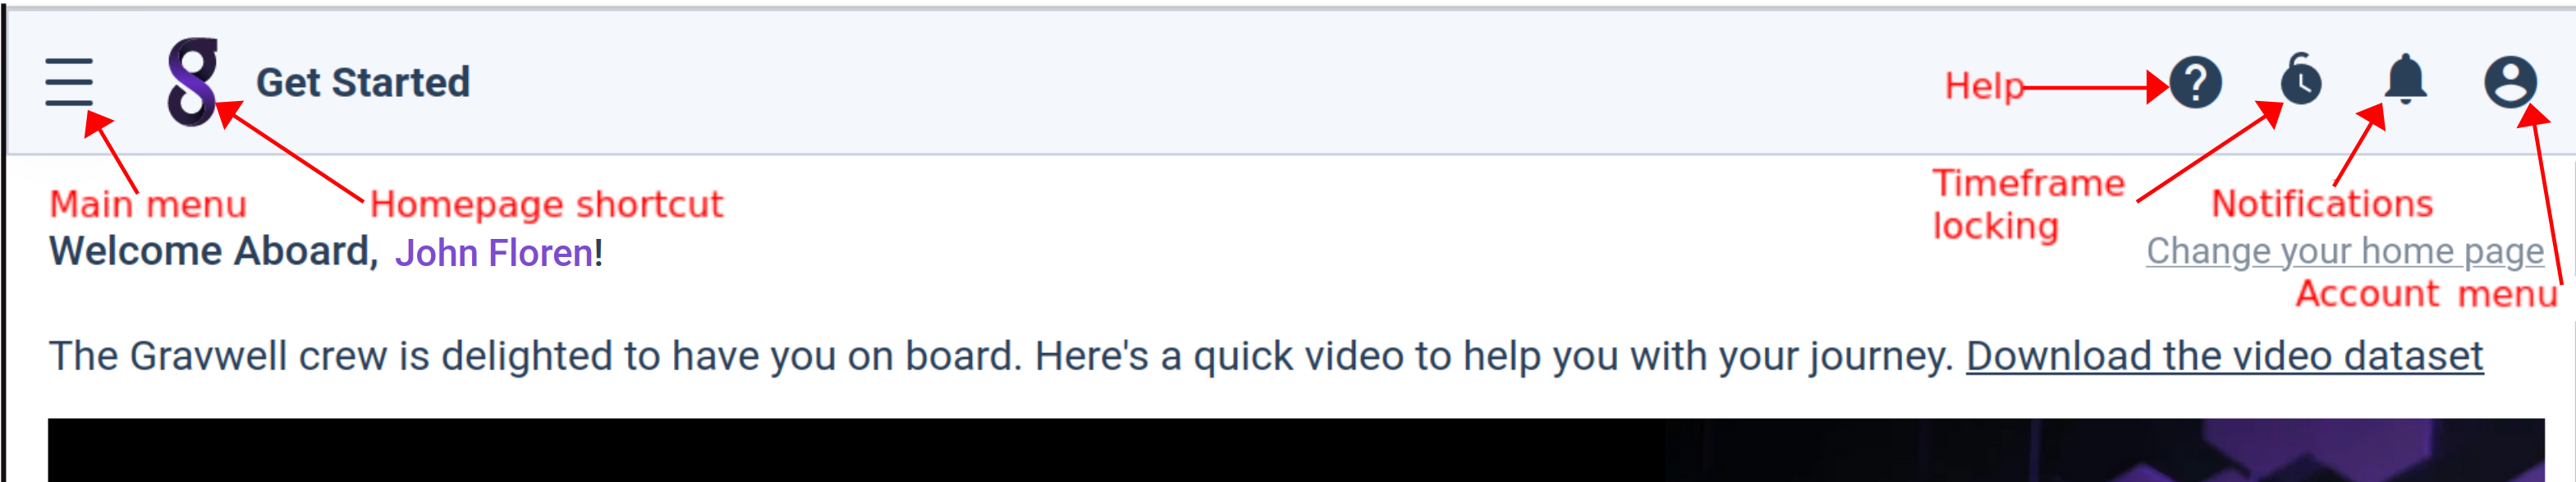
\includegraphics{images/homepage.png}
	\caption{Default home page}
	\label{fig:newsearch}
\end{figure}

Clicking the Gravwell logo in the upper left will always take you back to your home page (see section \ref{sec:account-menu} for configuration options).

\subsection{The Main Menu}
\index{GUI!main menu}

Clicking the ``hamburger'' button in the upper left will open the Main Menu, as shown in Figure \ref{fig:mainmenu}.

\begin{figure}
	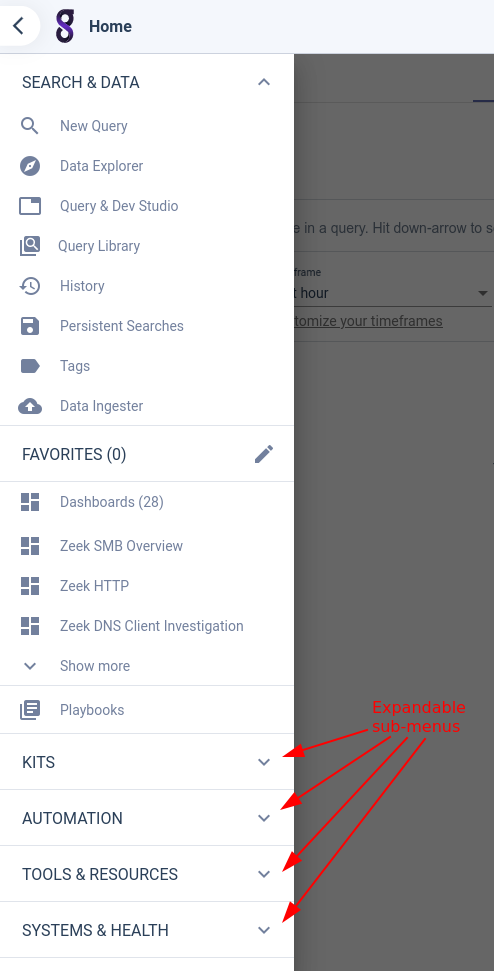
\includegraphics[width=0.45\linewidth]{images/menu.png}
	\caption{The main menu}
	\label{fig:mainmenu}
\end{figure}

This menu is used to access all the primary functionalities of Gravwell, including dashboards, the query library, and playbooks. Note that several items within the menu are actually sub-menus, which can be expanded to show additional options as shown in Figure \ref{fig:submenu}. Items within these sub-menus will typically be used less frequently that the top-level items and are therefore collapsed to save space.

\begin{figure}
	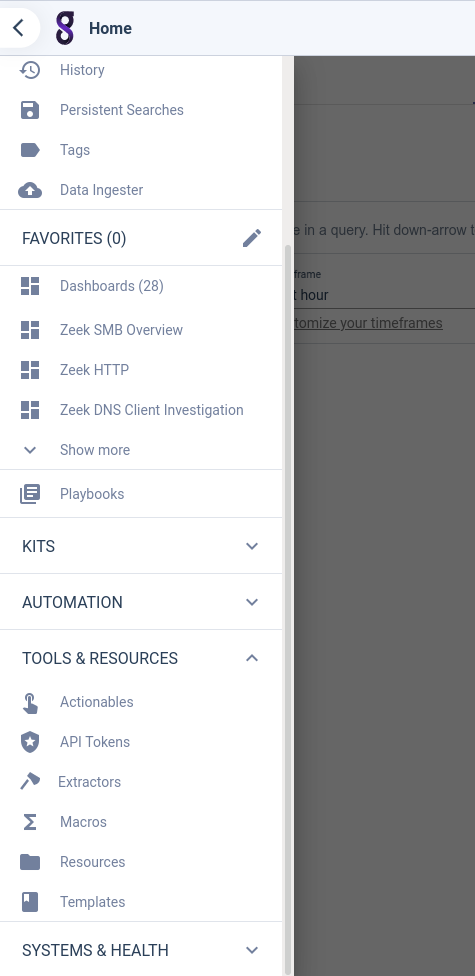
\includegraphics[width=0.45\linewidth]{images/menu-expanded.png}
	\caption{Expanded submenu}
	\label{fig:submenu}
\end{figure}

\clearpage

\subsection{Notifications}
\index{GUI!notifications}\index{Notifications}
Important notifications are accessible under the bell icon in the upper right corner of the page. Regular notifications are indicated by a small red circle containing the number of notifications. A critical notification will change the entire icon to a more attention-catching red icon; see Figure \ref{fig:notifications-icons} for examples.

\begin{figure}
	
\includegraphics{images/notif-normal.png}
	
\includegraphics{images/notif-severe.png}
	\caption{Notification icons, normal (left) and critical (right)}
	\label{fig:notifications-icons}
\end{figure}

Clicking the notification icon will display the text of the notifications, as seen in Figure \ref{fig:notification-menu}. Clicking the ``snooze'' button on a notification will remove that notification from counter shown on the icon; this can be useful to prevent distractions.

Depending on the type of notification, clicking the ``delete'' icon may clear the notification entirely. Some notifications are persistent and cannot be deleted; some are system-wide and can only be deleted by the administrator, and some are targeted at the current user and can be deleted by that user. Note that there is no harm in clicking ``delete'' on a notification the user isn't allowed to delete.

\begin{figure}
	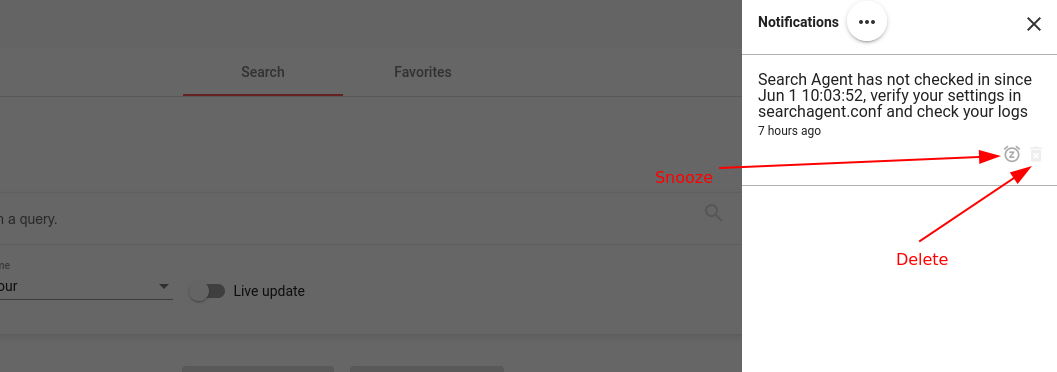
\includegraphics{images/notification-menu.png}
	\caption{Notifications menu}
	\label{fig:notification-menu}
\end{figure}

\clearpage
\subsection{The Account Menu}
\label{sec:account-menu}\index{GUI!account preferences}

The round button in the upper-right of the page is the Account Menu button. It will display either the initials of the current user, or a profile image if set. Clicking it brings up a small drop-down menu (Figure \ref{fig:accountmenu}).

\begin{figure}
	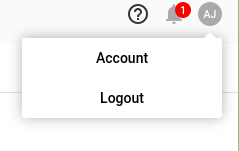
\includegraphics{images/user-dropdown.png}
	\caption{The account menu}
	\label{fig:accountmenu}
\end{figure}

Selecting ``Account'' will open your preferences page, shown in Figure \ref{fig:account-prefs}. Here, you can change your email address, display name, or password; be sure to click ``Update Account'' after making changes! The ``Log out all sessions'' button at the bottom of the screen will kick \emph{all} active sessions for your account, across all client machines.

\begin{figure}
	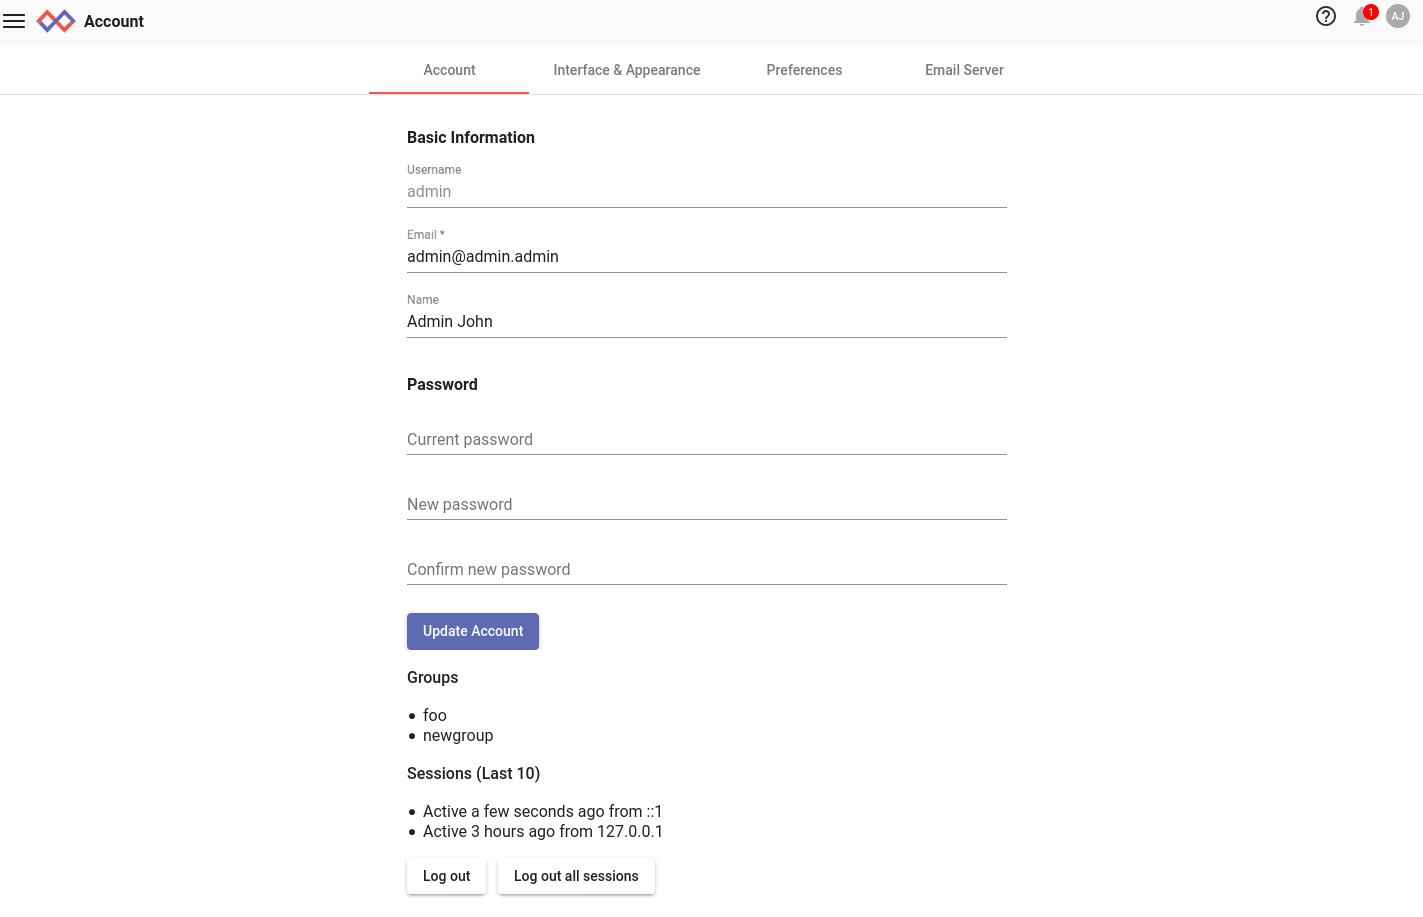
\includegraphics[width=0.7\linewidth]{images/account-prefs.png}
	\caption{Account preferences}
	\label{fig:account-prefs}
\end{figure}

The second tab of the Preferences page, ``Interface \& Appearance'', is shown in Figure \ref{fig:interface-prefs}. It has options for customizing the Gravwell user interface. The ``Interface theme'' dropdown is of particular interest, as it selects a GUI-wide color scheme (including the ever-popular dark modes). 

The ``Chart theme'' dropdown selects different color palettes which will be used when drawing charts. The editor theme \& font size options control the appearance of Gravwell's built-in text editor, which is used to create automation scripts and in a few other places.

\begin{figure}
	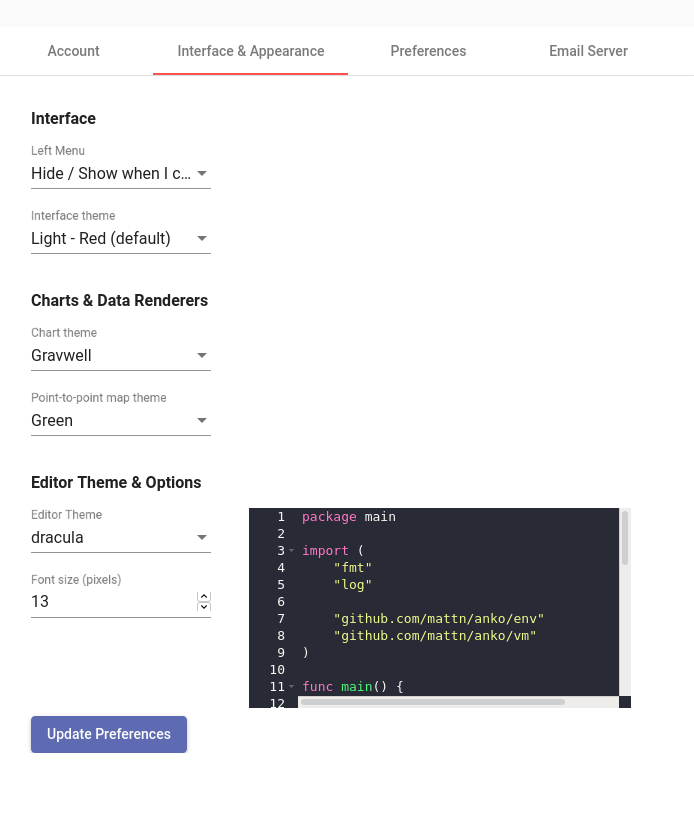
\includegraphics[width=0.7\linewidth]{images/interface-prefs.png}
	\caption{Interface and appearance preferences}
	\label{fig:interface-prefs}
\end{figure}

The third tab, ``Preferences'' (Figure \ref{fig:general-prefs}), allows you to change some default behaviors of Gravwell.

\begin{figure}
	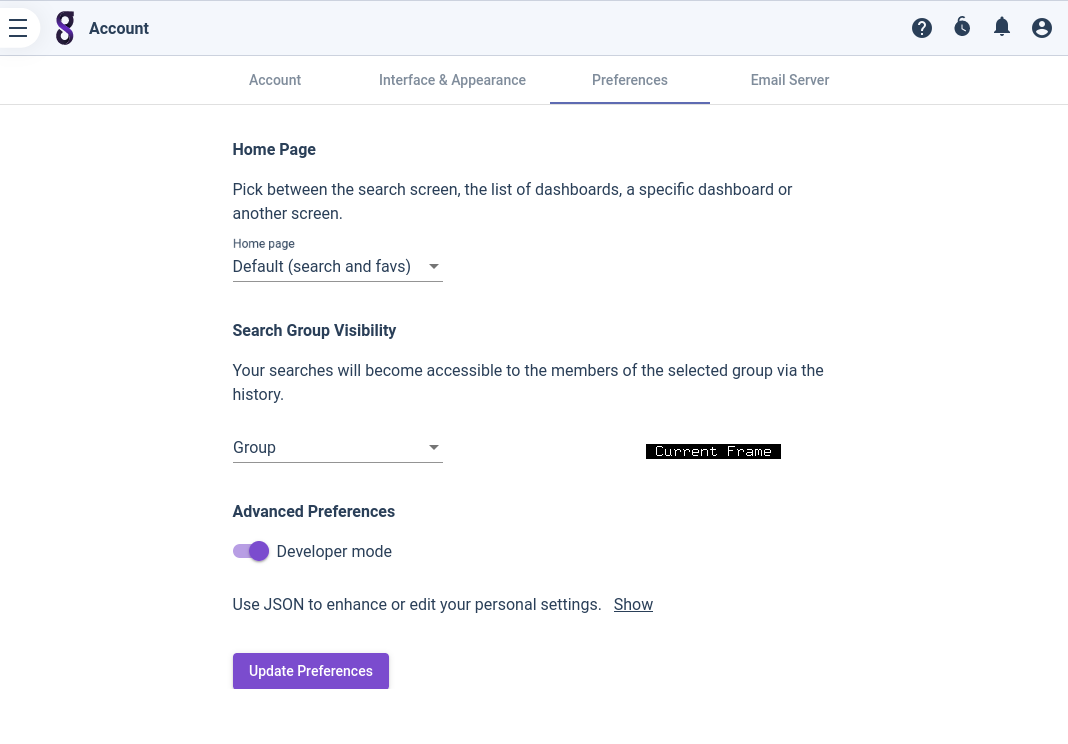
\includegraphics[width=0.7\linewidth]{images/general-prefs.png}
	\caption{General preferences}
	\label{fig:general-prefs}
\end{figure}


The ``Home Page'' dropdown menu selects which page will be displayed after logging in or clicking the Gravwell icon next to the main menu. By default, the welcome page is shown, but you can chose to be shown a list of dashboards, kits, or playbooks instead.

The ``Search Group Visibility'' option allows you to share the results of all searches with a given group; this can be a convenient way to collaborate. In the screenshot, the user has selected the group named ``foo''; all members of that group will have access to the searches this user runs in the future.

The ``Advanced Preferences'' section can be ignored by most users. Selecting ``Developer mode'' enables manual editing of JSON preferences.

The final tab, ``Email Server''\index{GUI!email configuration}\index{Email configuration} (Figure \ref{fig:email-prefs-gui}, is extremely important for users who intend to do automated email alerting via scheduled scripts. It must be set up with a valid SMTP configuration before emails can be sent.

\begin{figure}
	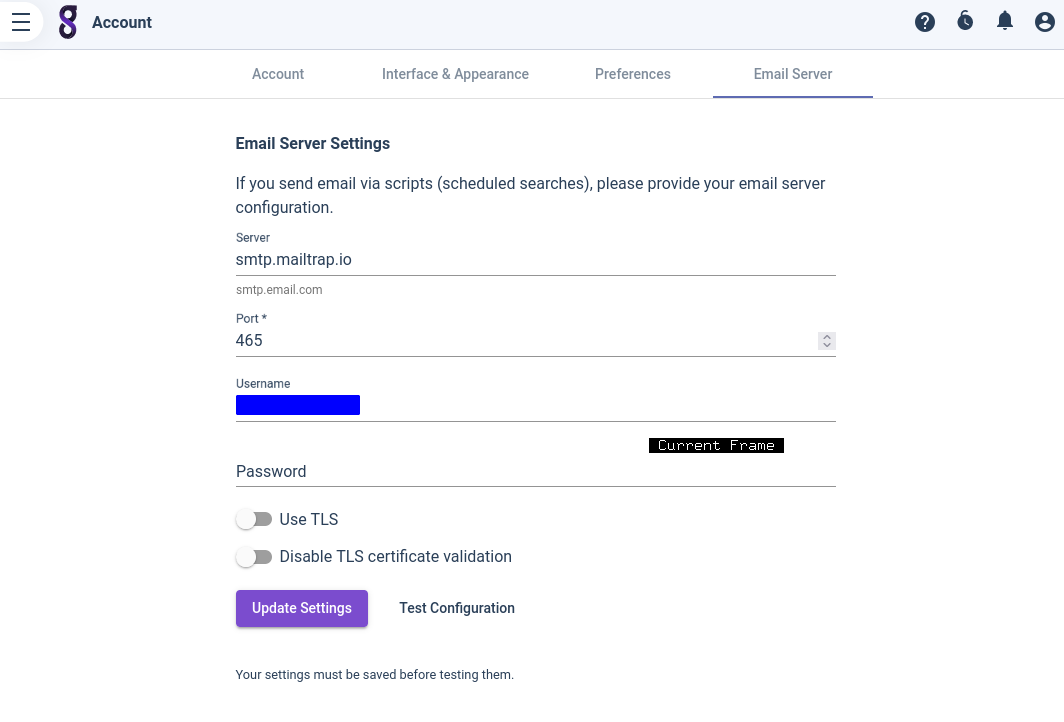
\includegraphics[width=0.7\linewidth]{images/email-prefs.png}
	\caption{Email preferences}
	\label{fig:email-prefs-gui}
\end{figure}

The fields are mostly self-explanatory; ``Server'' is an SMTP server, ``Port'' is the port to use for SMTP, ``Username'' and ``Password'' authenticate to that server. ``Use TLS'' should be enabled if the server expects TLS connections. The ``Disable TLS certification validation'' option is provided in case the server is using self-signed certificates; be cautious enabling this!

Once the fields have been populated, click ``Update Settings'' to save them, then click ``Test Configuration'' to send a test email.

\clearpage
\section{Labels and Filtering}
\index{GUI!labels}\index{Labels}
Objects in Gravwell such as dashboards, resources, macros, etc. can be labeled for organizational purposes. Some objects distributed in kits may be pre-labeled for convenience. The following object types can be labeled:

\begin{itemize}
\tightlist
\item Extractors
\item Dashboards
\item Kits
\item Playbooks
\item Resources
\item Scheduled Searches / Automation Scripts
\item Macros
\item Templates
\item Actionables
\item Query Library entries
\item User files
\end{itemize}

\subsection{Defining and Managing Labels}

Labels are added or deleted in the edit dialog for a given object. While the exact layout of the dialog varies for each object type, they will all have a section for Labels. Labels are added by typing the label into the text bar and hitting enter. Multiple labels can be added in succession in this manner. In Figure \ref{fig:resource-labels}, the user has added three labels (\code{network}, \code{asn}, and \code{lookup}) to a resource.

Labels may be removed in the edit dialog by clicking the ``x'' next to the label, or by using the backspace key.

\begin{figure}
	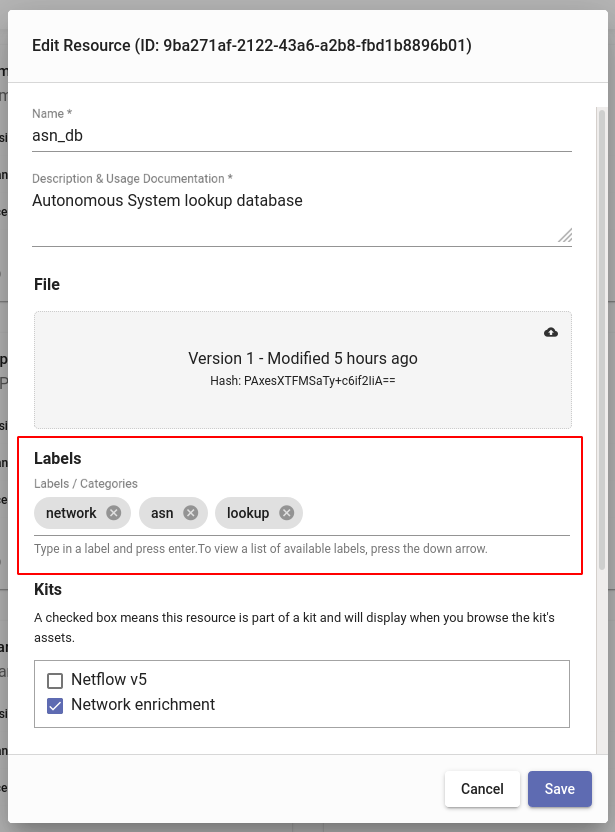
\includegraphics[width=0.5\linewidth]{images/resource-labels.png}
	\caption{Labels applied to a resource}
	\label{fig:resource-labels}
\end{figure}

\subsection{Filtering Objects}

The GUI can filter objects based on their labels. At the top of many screens is a bar containing a ``Filters'' button, as shown in Figure \ref{fig:filters-menu}. Clicking that button brings up a menu with several options for filtering (Fig \ref{fig:filters-options}).

Multiple filters can be applied simultaneously. When a filter has been applied to a page, a blue ``X'' icon will appear on the Filters button. Clicking this icon will clear all filters.

\begin{figure}
	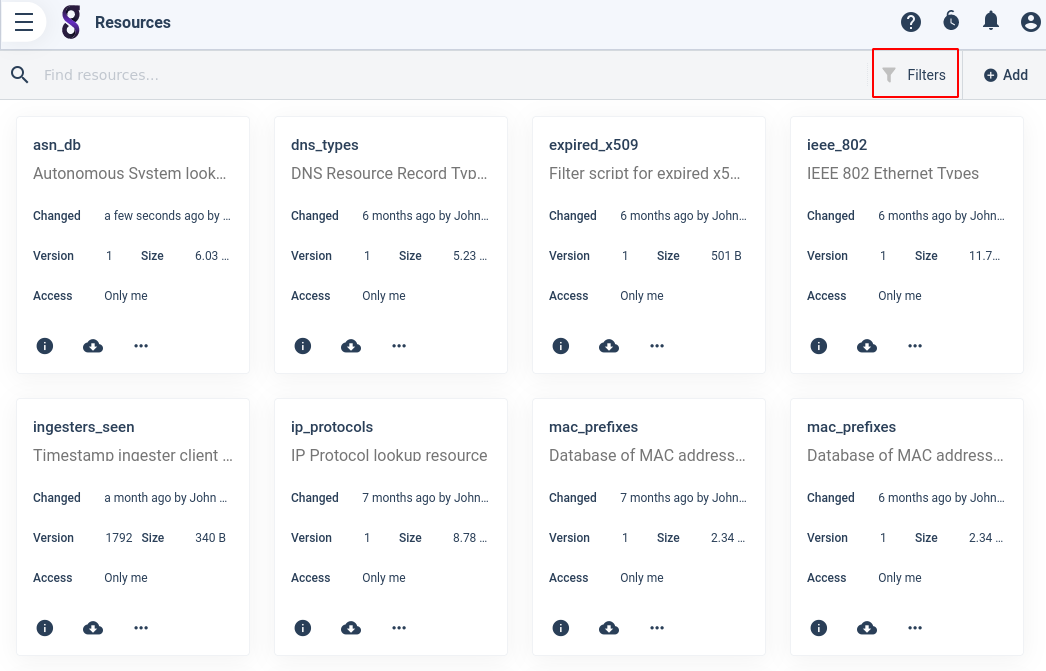
\includegraphics[width=0.7\linewidth]{images/filters-menu.png}
	\caption{The filters menu}
	\label{fig:filters-menu}
\end{figure}

\begin{figure}
	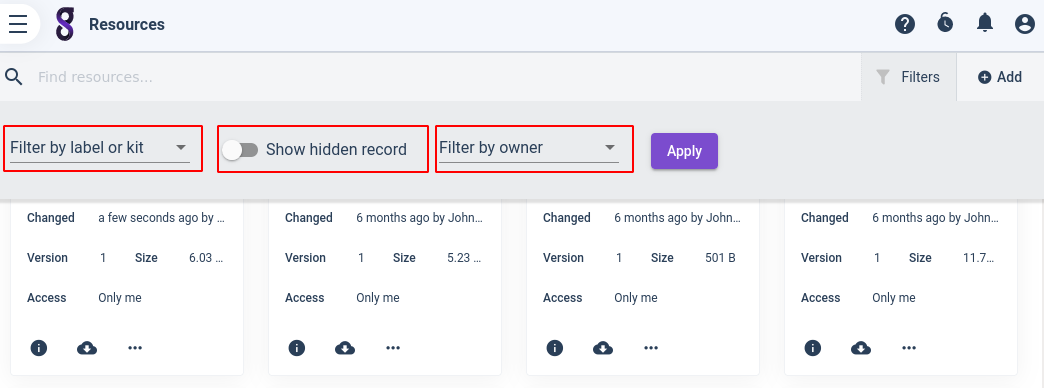
\includegraphics[width=0.7\linewidth]{images/filters-options.png}
	\caption{Options for filtering}
	\label{fig:filters-options}
\end{figure}

\subsubsection{Filtering by Label}

The left-most dropdown, ``Filter by label or kit'', allows you to select one or more labels or kits. Clicking the Apply button will then show only those objects with the specified labels or installed by the specified kits. Figure \ref{fig:filter-labels} shows the user selecting the ``lookup'' label, which will hide all resources not labeled ``lookup''.

\begin{figure}
	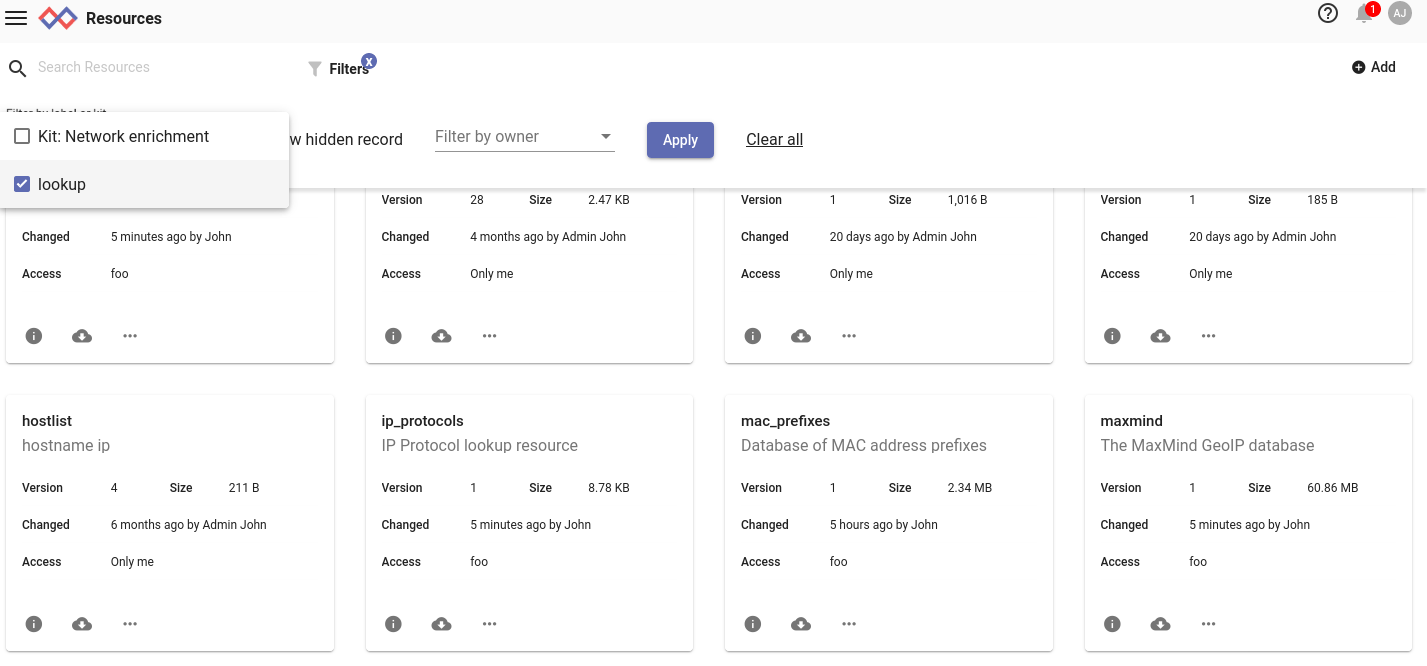
\includegraphics[width=0.8\linewidth]{images/filter-labels.png}
	\caption{Filtering by label}
	\label{fig:filter-labels}
\end{figure}

\subsubsection{Filtering by Owner}

By default, most interfaces will show all objects the user has access to, regardless of owner. Another filter option can make it show only objects owned by a particular set of users. Figure \ref{fig:filter-owner} shows the user filtering macros to show only those macros owned by the user named ``Admin User''. Note that the ``My data'' option applies to the current user; selecting this checkbox will show only those items which \emph{belong} to the current user, rather than all items the user \emph{can access}.

\begin{figure}
	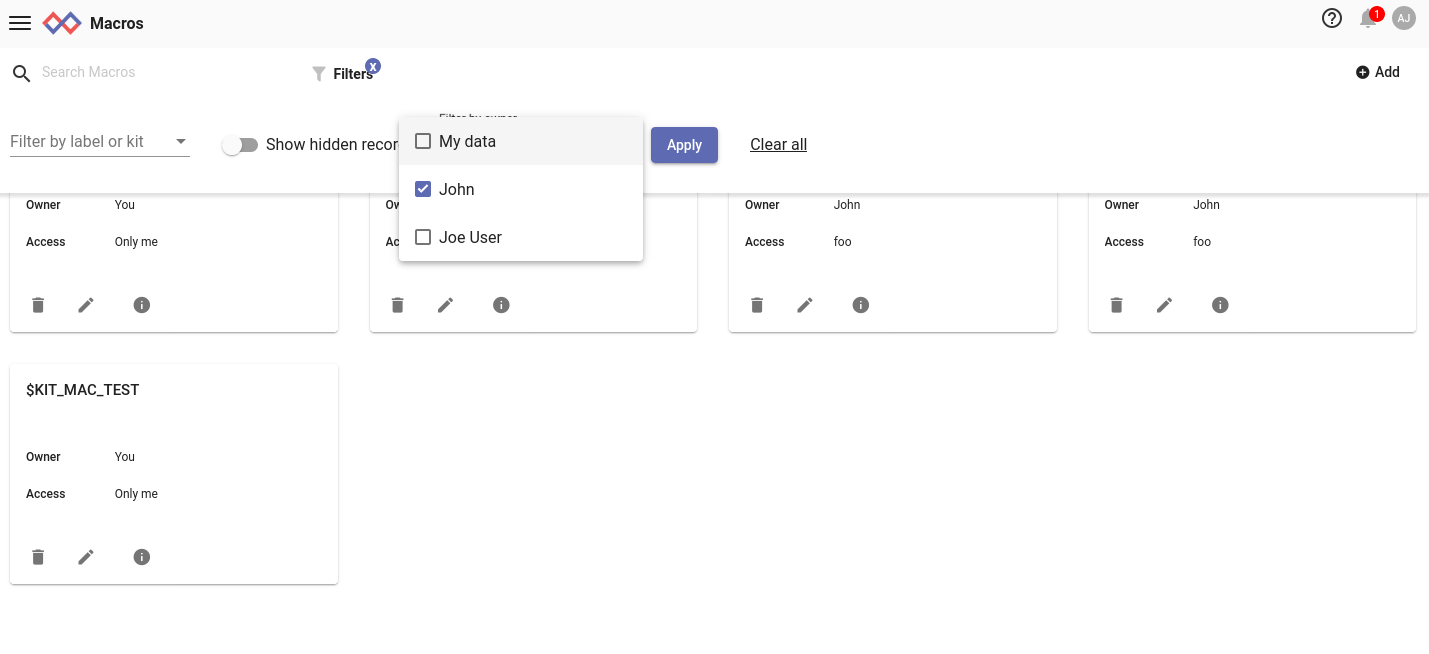
\includegraphics[width=0.8\linewidth]{images/filter-owner.png}
	\caption{Filtering by owner}
	\label{fig:filter-owner}
\end{figure}

\subsubsection{Showing Hidden Objects}

Objects with the special label \code{hidden} are not displayed by default. This is a convenience function which can keep displays clear of rarely-accessed objects. Click the ``Show hidden record'' toggle to show hidden objects. In Figures \ref{fig:filter-hidden} and \ref{fig:filter-hidden-applied}, toggling ``Show hidden record'' reveals an additional hidden macro.

\begin{figure}
	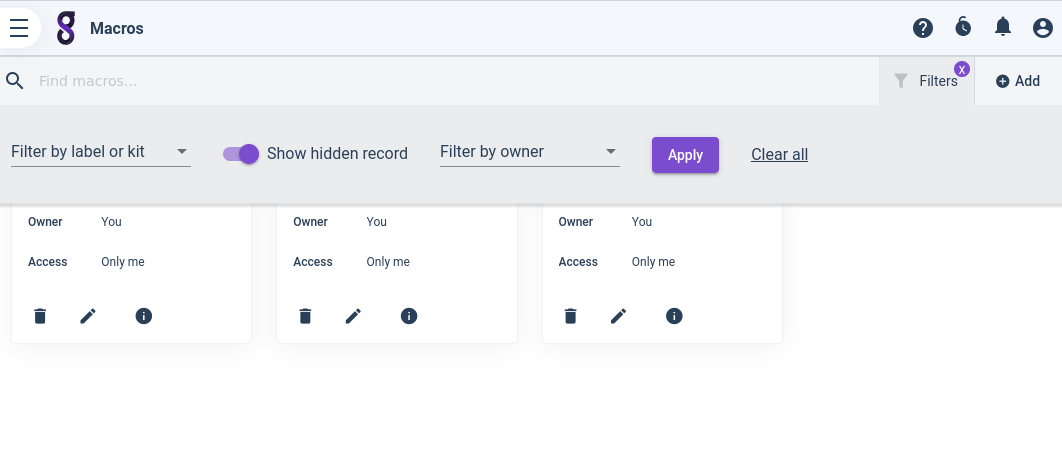
\includegraphics[width=0.6\linewidth]{images/filter-hidden.png}
	\caption{Enabling the ``show hidden'' toggle}
	\label{fig:filter-hidden}
\end{figure}

\begin{figure}
	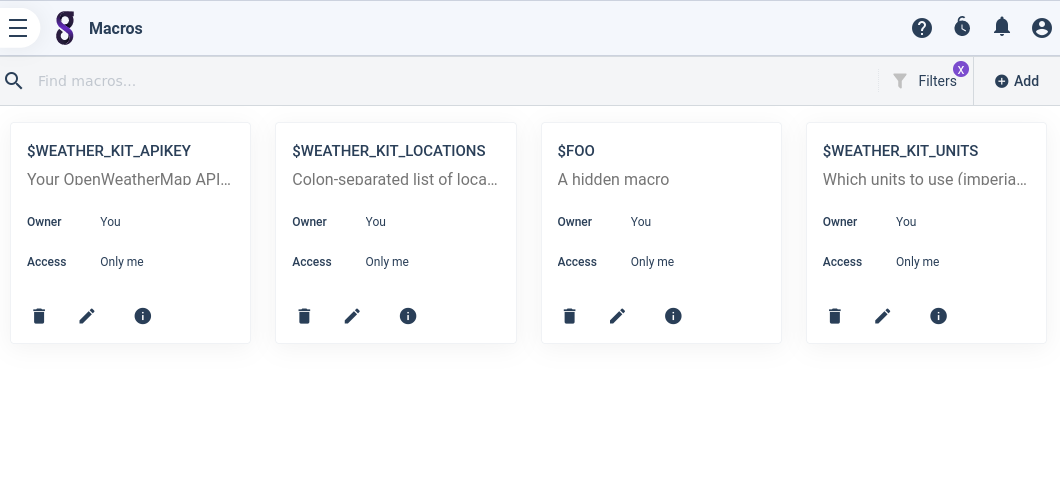
\includegraphics[width=0.6\linewidth]{images/filter-hidden-applied.png}
	\caption{Hidden item becomes visible with ``show hidden'' enabled}
	\label{fig:filter-hidden-applied}
\end{figure}

\clearpage

\subsection{Special Labels}

Gravwell defines a handful of special labels and label prefixes for particular operations.

The string \code{hidden} is a special label; applying it to an object will prevent the object from being displayed by default. To see the object, toggle the ``Show hidden record'' option in the filter menu, as detailed above.

\subsubsection{Kit Label Prefixes}
\index{Kits!kit labels}
Three label prefixes are used to manage Gravwell-internal information about objects which were installed as part of a kit. You should never manually apply kit labels to objects; these labels are documented to prevent users from accidentally applying a conflicting label to an object. The following are considered reserved kit label prefixes:


\begin{itemize}
\tightlist
\item kit/
\item kit/dependency:
\item kit/configuration:
\end{itemize}

Users should not create labels beginning with these strings, e.g. \code{kit/foo} or \code{kit/dependency:bar}. These labels are managed internally by Gravwell.

\clearpage
\section{Search Interfaces}
\label{sec:search-interfaces}
\index{Search}
There are two different user interfaces for running searches in Gravwell: the classic lightweight search interface, and the multi-tabbed Query Studio. Which should you use? Either is acceptable, both take exactly the same Gravwell queries, but most users will find the Query Studio most comfortable.

Throughout this text, screenshots may use either interface interchangeably, because they are \emph{designed} to be used interchangeably. Every feature available in the classic interface is available in the Query Studio. The Query Studio provides a few extra conveniences (including more advanced Data Explorer functionality (Section \ref{sec:data-explorer}), which is why we recommend it to most users.

The classic search interface is accessed via the ``New Query'' option in the main menu. It presents a very sparse and straightforward way to enter a Gravwell query, along with a few options such as timeframe selection (Figure \ref{fig:original-search}).

\begin{figure}
	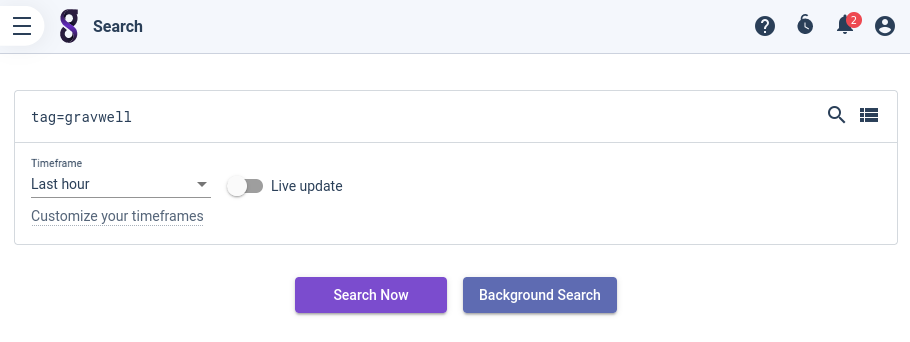
\includegraphics[width=0.8\linewidth]{images/original-search.png}
	\caption{The classic search interface}
	\label{fig:original-search}
\end{figure}

Clicking ``Search Now'' launches the search, taking the user to the classic results page as seen in Figure \ref{fig:original-results}. From here, the query can be modified and iterated on, re-running the search again and again as you explore data.

\begin{figure}
	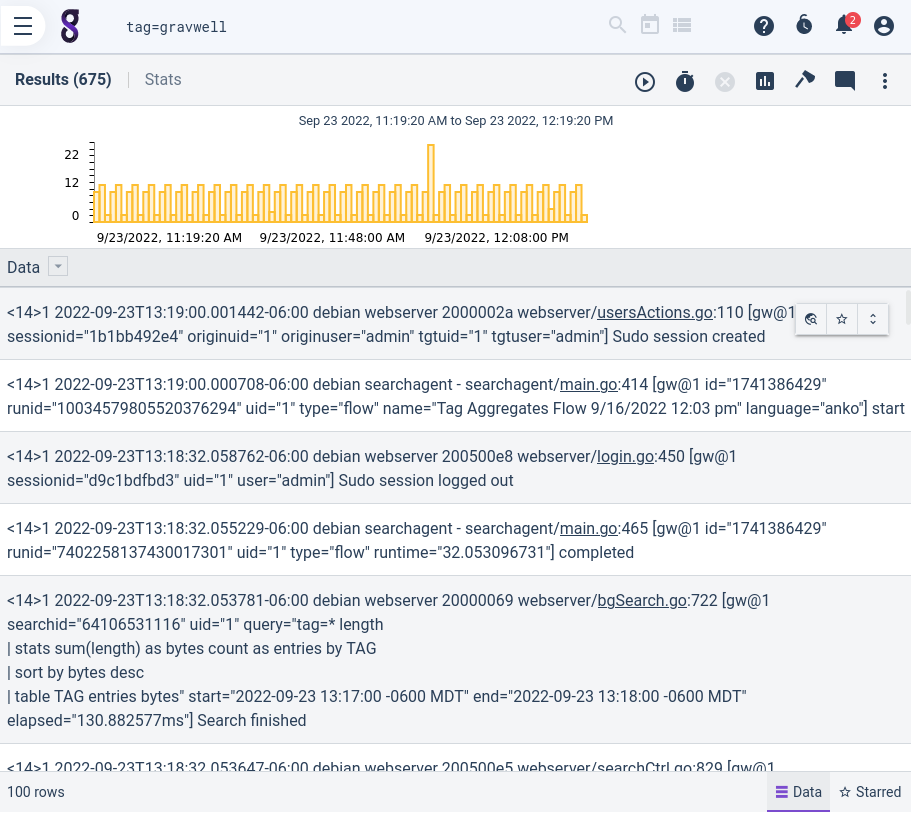
\includegraphics[width=0.9\linewidth]{images/original-results.png}
	\caption{The classic search results page}
	\label{fig:original-results}
\end{figure}

The Query Studio is a newer interface, designed to provide a convenient multi-tabbed environment in which a user can work with multiple queries at the same time. Figure \ref{fig:query-studio} shows what the Query Studio looks like when first opened. Note how it presents a list of queries from the query library, templates, and selections from recent query history; clicking any of these will launch the selected query. Clicking ``Start a New Query'' begins with a blank query instead.

\begin{figure}
	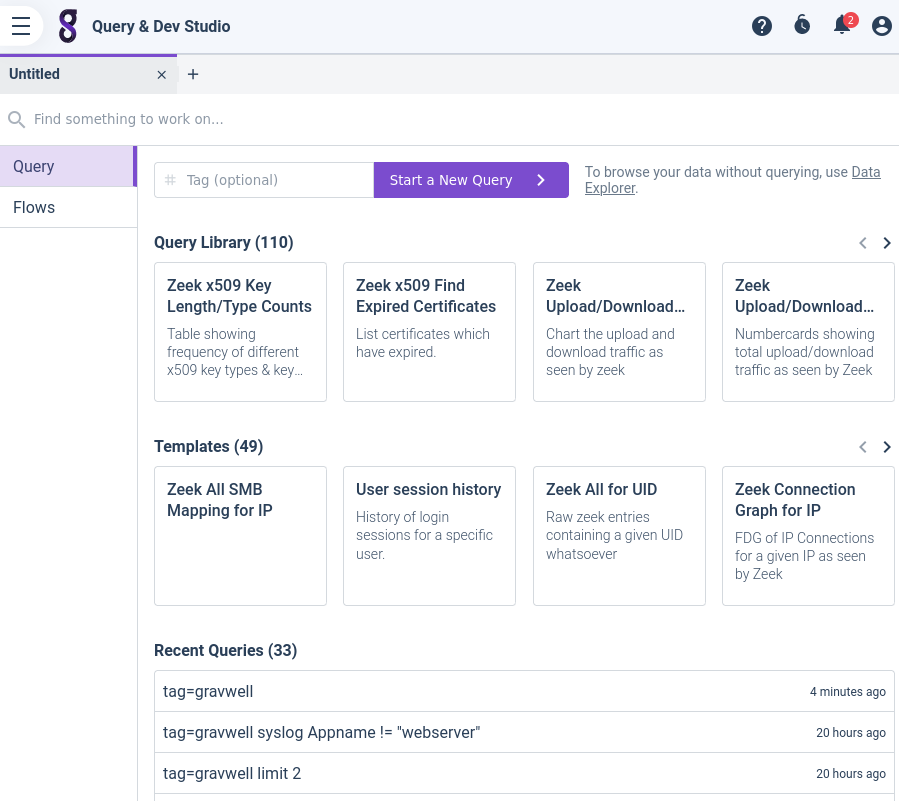
\includegraphics[width=0.9\linewidth]{images/query-studio.png}
	\caption{The Query Studio}
	\label{fig:query-studio}
\end{figure}

Figure \ref{fig:query-studio-results} shows the Query Studio with two tabs open. The current tab displays the results of a chart query. Note the ``Pie Chart'' text near the upper right; this is a drop-down menu which allows the user to quickly change between chart types when running a query with the chart renderer. This and other conveniences make the Query Studio a more comfortable environment for most users.

\begin{figure}
	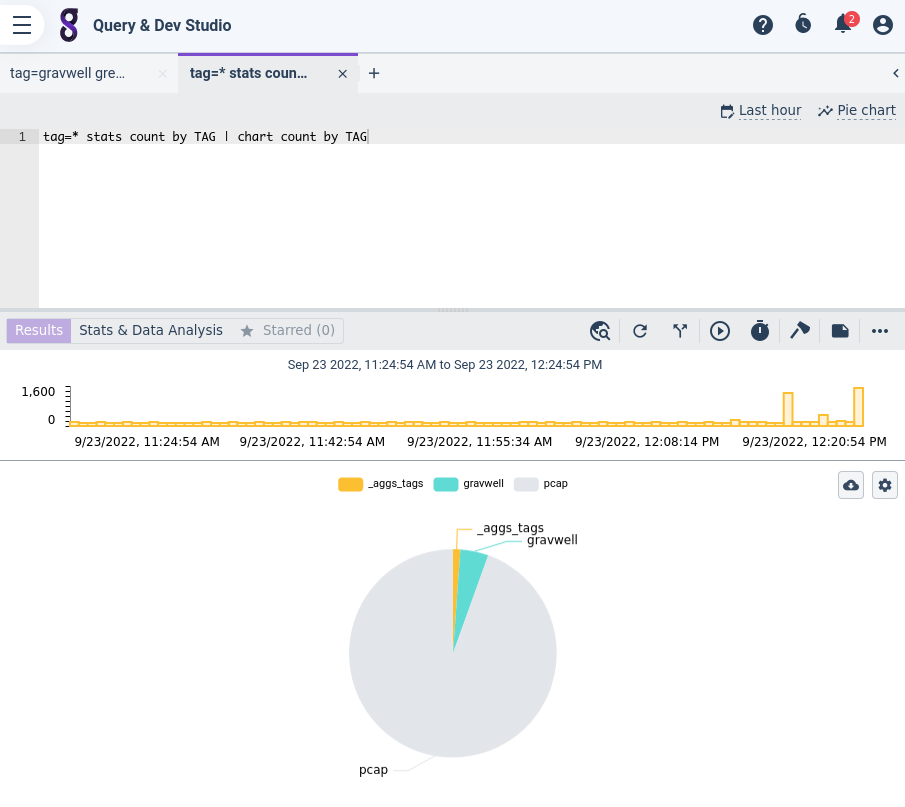
\includegraphics[width=0.9\linewidth]{images/query-studio-results.png}
	\caption{Query Studio results display}
	\label{fig:query-studio-results}
\end{figure}

\clearpage
\section{Playbooks}
\index{Playbooks}
Playbooks are hypertext documents within Gravwell which help guide users through common tasks, describe functionality, and record information about data in the system. Most Gravwell kits (see Chapter \ref{ch:kits}) include a playbook or two to help users get oriented in the kit, but regular users can also \emph{create} playbooks for themselves, documenting their data investigations with a mix of text, images, and \emph{executable queries}.

The Playbooks page (Figure \ref{fig:playbooks}) lists the playbooks currently in the system and allows the creation of new ones.

\begin{figure}
	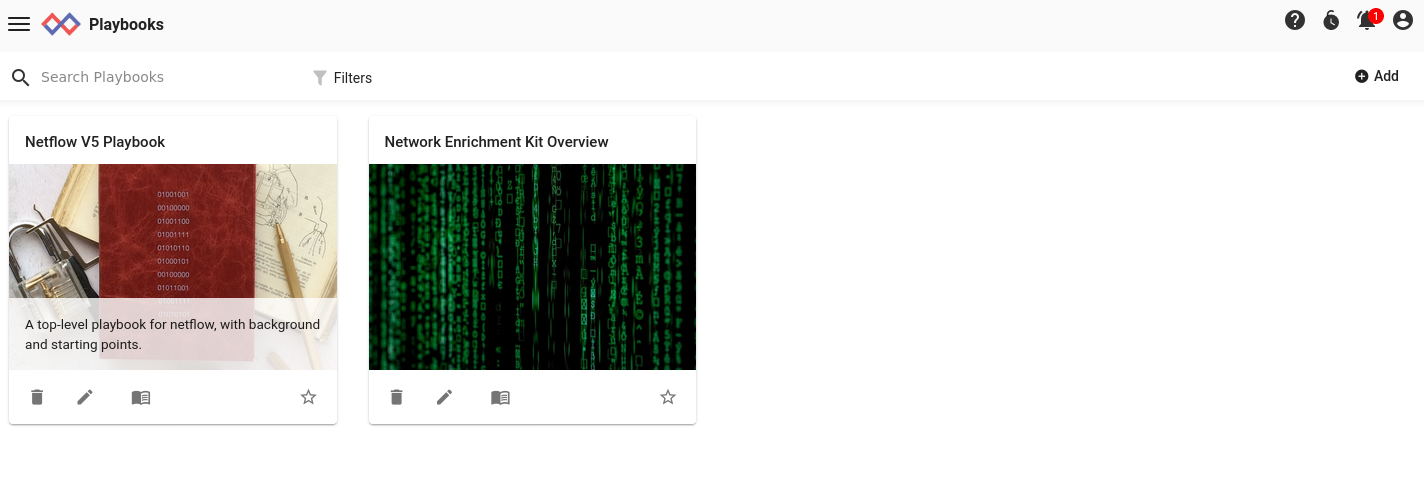
\includegraphics[width=0.8\linewidth]{images/playbooks.png}
	\caption{Playbooks page}
	\label{fig:playbooks}
\end{figure}

Clicking a playbook will open it. It will look more or less like a regular web page, with section headings, hyperlinks, and images, but it will also include embedded queries, as seen in Figure \ref{fig:playbook-read}. Clicking the `Launch' button will run that query in a new browser tab.

\begin{figure}
	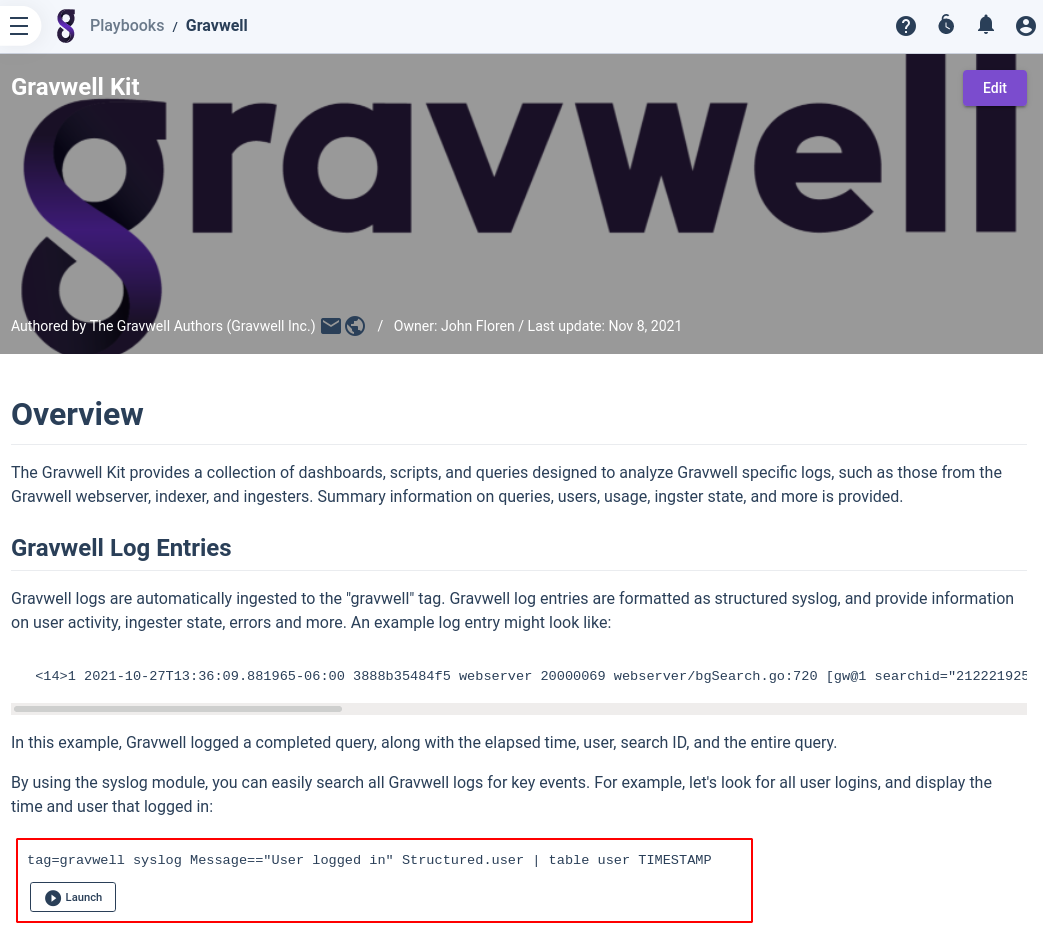
\includegraphics[width=0.8\linewidth]{images/playbook-read.png}
	\caption{Playbook viewer}
	\label{fig:playbook-read}
\end{figure}

\subsection{Playbook Markdown}
\index{Markdown}
Playbooks are written in Markdown. You can edit an existing playbook by clicking the edit button, or create your own new playbook. This will bring up an editor as shown in Figure \ref{fig:playbook-edit}

\begin{figure}
	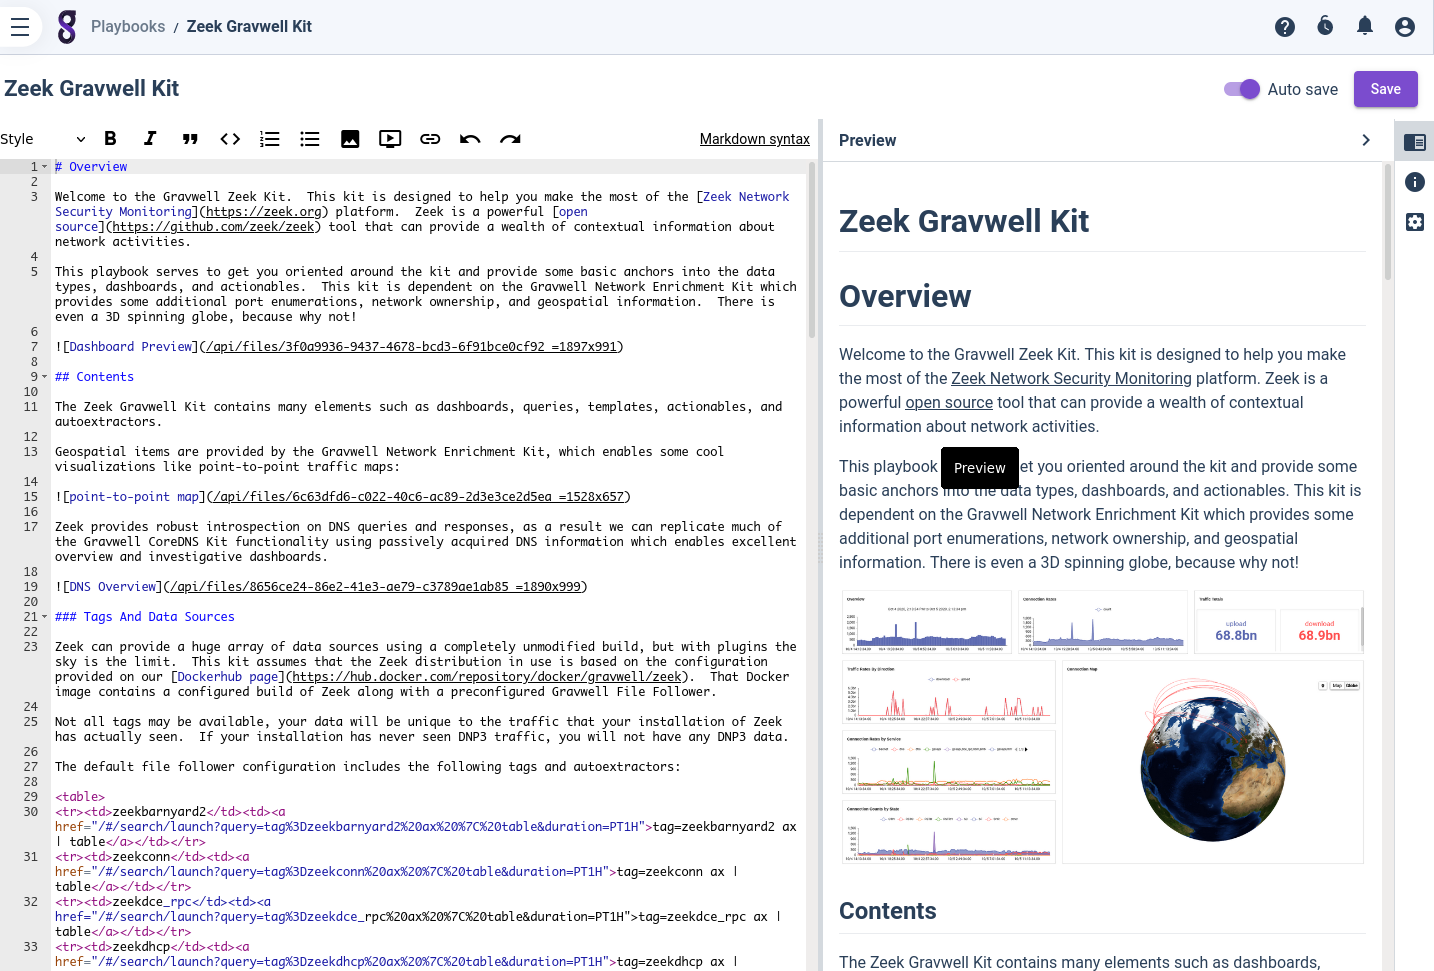
\includegraphics[width=0.8\linewidth]{images/playbook-edit.png}
	\caption{Playbook editor}
	\label{fig:playbook-edit}
\end{figure}

The editor accepts standard Markdown syntax\footnote{https://www.markdownguide.org/basic-syntax/}:

\begin{itemize}
\item Designate headings with number signs (\#), using one for heading level 1, two for heading level 2, and so on, e.g. \code{\# Heading 1}, \code{\#\#\# Heading 3}.
\item Surround text with asterisks to italicize, or with doubled asterisks to bold, e.g. \code{*italic*}, \code{**bold**}.
\item Hyperlinks put the link text in square brackets and the target URL in parentheses: \code{[Example Site](http://example.com)}
\item Create numbered lists by numbering each line (\code{1. First item} and so on), create bulleted lists with asterisks (\code{* First item}).
\end{itemize}

Review the full Markdown syntax document for more options. You can also insert plain old HTML if necessary. Note that there are two essential changes to the syntax which are explained below.

\subsubsection{Inserting Runnable Queries}

Playbooks can contain Gravwell queries which will be displayed with a ``Launch'' button for the user to click. To insert a query, use the Markdown blockquote syntax, as below:

\begin{verbatim}
```
tag=netflow netflow Protocol Src SrcPort Dst DstPort | table
```
\end{verbatim}

\subsubsection{Inserting Images}

Images can be inserted in two ways. The first is the standard Markdown method using a hyperlink:

\begin{verbatim}
![This is the image alt text](https://example.com/image.jpg)
\end{verbatim}

The other method involves uploading an image \emph{to Gravwell}. To do this, click the `Add image' icon in the playbook editor. The UI will prompt you to upload an image as seen in Figure \ref{fig:playbook-upload}. Once you select a file to upload, the dialog will prompt you for alt text and other information as shown in Figure \ref{fig:playbook-upload2}. Once you click `Add', the editor will insert Markdown code referring to your newly-uploaded file within Gravwell:

\begin{verbatim}
![A cat](/api/files/c39a9541-971f-44b1-97ac-5724d5214f05 =1240x698)
\end{verbatim}

\begin{figure}[H]
	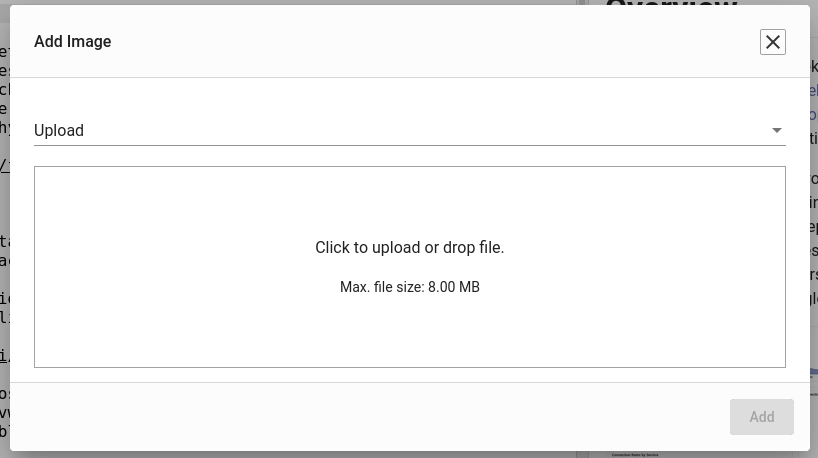
\includegraphics[width=0.6\linewidth]{images/playbook-upload.png}
	\caption{Playbook image upload}
	\label{fig:playbook-upload}
\end{figure}

\begin{figure}[H]
	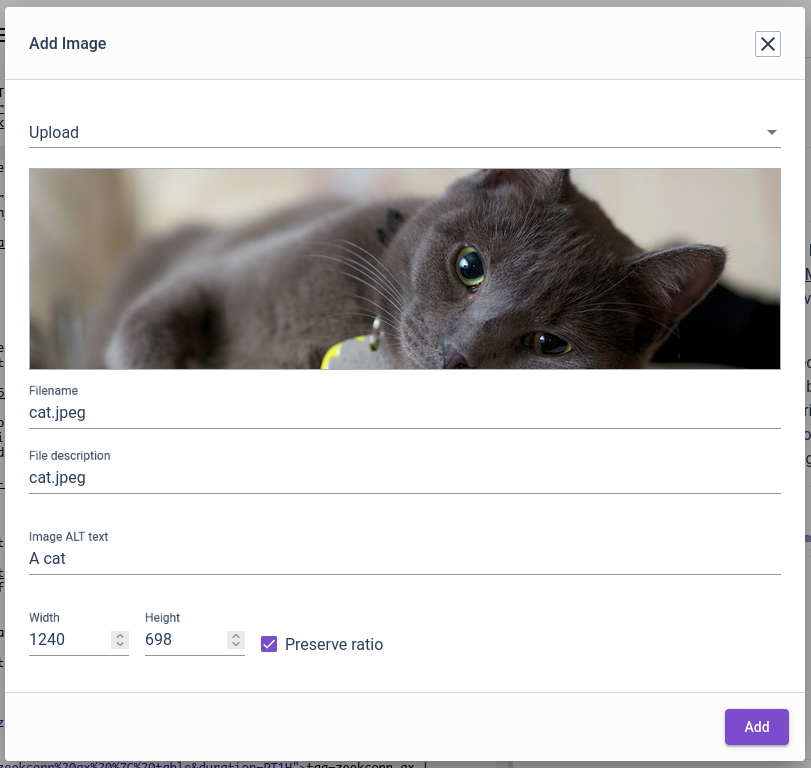
\includegraphics[width=0.6\linewidth]{images/playbook-upload2.png}
	\caption{Playbook image upload}
	\label{fig:playbook-upload2}
\end{figure}

You can also insert a previously-uploaded image by selecting `Gallery' in the dialog's drop-down menu, as shown in Figure \ref{fig:playbook-gallery}.

\begin{figure}[H]
	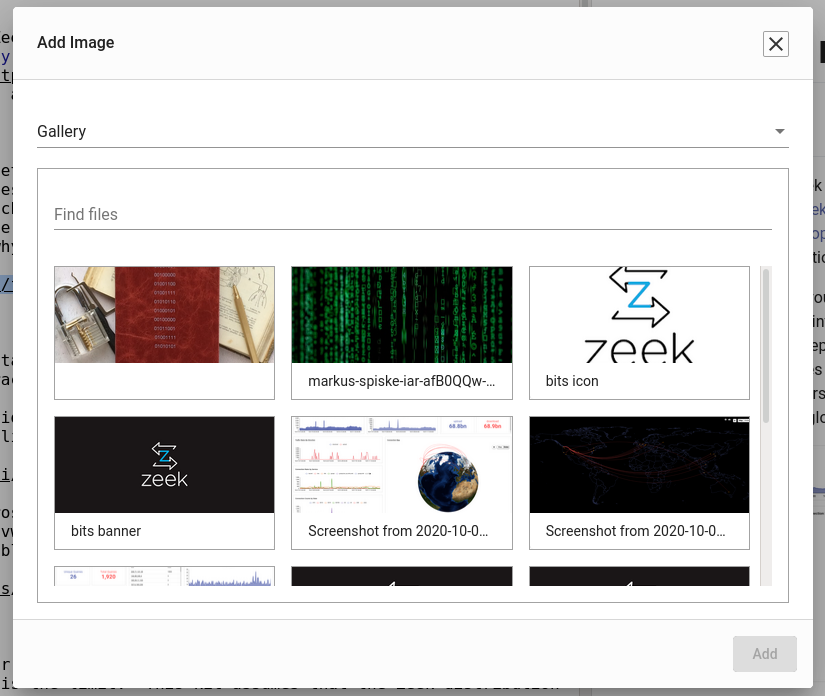
\includegraphics[width=0.6\linewidth]{images/playbook-gallery.png}
	\caption{Playbook image gallery}
	\label{fig:playbook-gallery}
\end{figure}
